\documentclass{standalone}
\usepackage{pgfplots}
\begin{document}
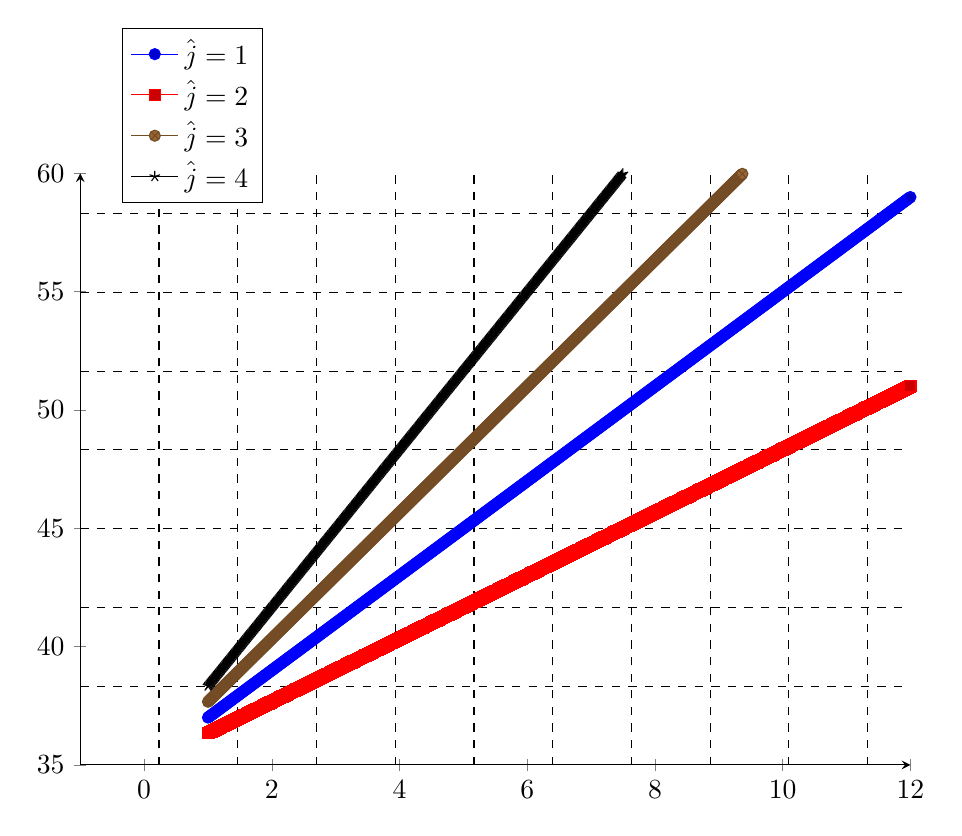
\begin{tikzpicture}
    \begin{axis}[width=\textwidth,height=0.75\textwidth,
        xmin=-1,xmax=12,ymin=35,ymax=60,samples=1000,
        legend style={at={(0.05,0.95)},anchor=south west},
        axis x line=center, axis y line=left]
    \draw[dashed] (\pgfkeysvalueof{/pgfplots/xmin},\pgfkeysvalueof{/pgfplots/ymin}) grid[step=1cm] 
        (\pgfkeysvalueof{/pgfplots/xmax},\pgfkeysvalueof{/pgfplots/ymax});
    \legend{$\hat{j}=1$,$\hat{j}=2$,$\hat{j}=3$,$\hat{j}=4$};
    \addplot+[domain=1:12,samples=1000] ({x},{2*x+35});
    \addplot+[domain=1:12,samples=1000] ({x},{(4/3)*x+35});
    \addplot+[domain=1:12,samples=1000] ({x},{(8/3)*x+35});
    \addplot+[domain=1:12,samples=1000] ({x},{(10/3)*x+35});
    \end{axis}
\end{tikzpicture}
\end{document}